{\color{indiagreen}\subsection{Agregatna stanja}}
Agregatna stanja:
\begin{itemize}
	\item trdnine zavzamejo svojo obliko, večja gostota, kot pri kapljevinah in tekočinah, delci med sabo so močno vezani
	\item kapjevine(tekočine) vedno zavzamejo spodnji del in tvorijo gladino, lahko tvorijo kapjice.
	\item plini(tekočine) zavzamejo celoten prostor
\end{itemize}
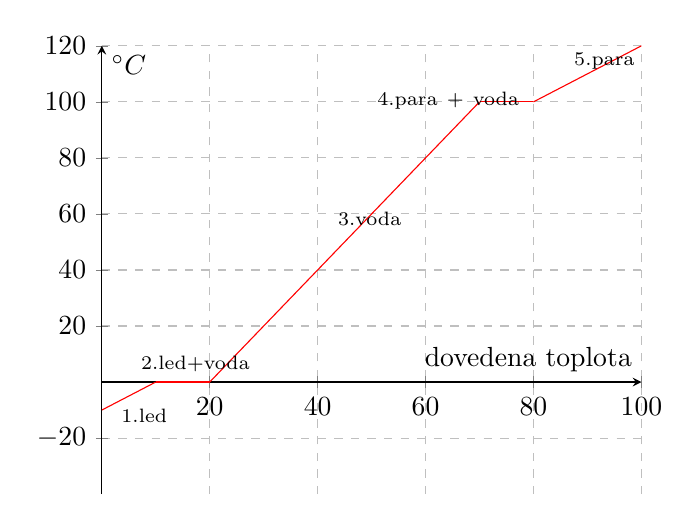
\begin{tikzpicture}
	\begin{axis}[
	    xlabel={dovedena toplota},
	    ylabel={$^{\circ}C$},
	    xmin=0, xmax=100,
	    ymin=-40, ymax=120,
	    xtick={0,20,40,60,80,100},
	    ytick={-20,0,20,40,60,80,100,120},
	    ymajorgrids=true,
	    xmajorgrids=true,
	    grid style=dashed,
	    axis lines=middle,
	]
	\addplot[domain=0:10,red] {x-10};
	\addplot[domain=10:20,red] {0};
	\addplot[domain=20:70,red] {2*x-40};
	\addplot[domain=70:80,red] {100};
	\addplot[domain=80:100,red] {x+20};
	\end{axis}

	\node[text width=1cm] at (0.75,1){\scriptsize {1.led}};
	\node[text width=1cm] at (1,1.65){\scriptsize{2.led+voda}};
	\node[text width=1cm] at (3.5,3.5){\scriptsize{3.voda}};
	\node[text width=3cm] at (5,5){\scriptsize{4.para + voda}};
	\node[text width=1cm] at (6.5,5.5){\scriptsize{5.para}};

\end{tikzpicture}
\textbf{LED $\rightarrow$ VODA $\rightarrow$ PARA}\\
\begin{enumerate}
	\item Segrevanje ledu\\
	\begin{align*}
		Q &= m c_l \Delta T\\
		c_l &= 2100 \frac{J}{kgK}\dots \text{specifična toplota ledu}\\
	\end{align*}
	\item Taljenje ledu: izotermen proces, ledišče (temperatura pri kateri se iz trdnega stanja spremeni v kapjevino)\\
	\begin{align*}
		Q &= q_t m\\
		q_t &\dots \text{specifična talilna toplota}\\
		q_t &= \frac{Q}{m}[1\frac{J}{kgK}]\\
		q_{tv} &= 333 \frac{kJ}{kgK}
	\end{align*}
	\item Segrevanje vode
	\begin{align*}
		Q &= m c_v \Delta T\\
		c_v &= 4200 \frac{J}{kgK}\\
	\end{align*}
	\item Vrenje(izparevanje): izotermen proces, temperatura pri kateri kapljevina vre pravimo vrelišče
	\begin{align*}
		Q &= m q_i\\
		q_i &\dots \text{specifična talilna toplota(koliko toplote potrebujemo, da izparimo 1 kg snovi)}\\
		q_i &= \frac{Q}{m}[1\frac{J}{kgK}]\\
		q_{iv} &= 2250 \frac{kJ}{kgK}\\
	\end{align*}
	\item Segrevanje pare
	\begin{align*}
		Q &= m c_p \Delta T\\
		c_p &= 2100 \frac{J}{kgK}\dots \text{specifična toplota pare}\\
	\end{align*}
\end{enumerate}
\textbf{latenta toplota $=$ specifična toplota}
